% !TEX root = ../main.tex

\chapter{Introduction}
\minitoc

% -- Rewrite sketch --
% BSP is big and important. Hero runs running large homogenous workloads. Massive costs.

% Two problems emerge from its tightly synchronized nature: data path and compute path

% Data path: checkpoint, fault tolerance or analysis

% Compute path: performance and correctness issues.

% First studies CARP as a data management problem: adaptive mechanism for range partitoining. Then placement in AMR codes as a
% compute path efficiency problem. CARP is a narrow success story: an adaptive mechanism
% built off a global repartitioning primitive worked. AMR experience highlights a broader class
% of unknowables.

% 1. How much telemetry you need from what source
% 2. When to intervene, what shape should the intervention take, did it work?
% 3. Tunables: no right answer

% Worse, no takeaway is portable. Every site has its own unique problems. You can't collect all telemetry and ship it somewhere else.

% There is a feedback loop here. You run, collect telemetry, analyze it, intervene. It is currently super slow.
% Fragmented tools. Need to run workload again and again. ETL bottleneck. Bad formats. No structure (rank-major vs timestep-major).
% Nature of unknowables + cost and fragility demands faster adaptive loops. Present ORCA is a general
% substrate for steerable observability and control.

% 2. Thesis Statement
% Efficiency in bulk-synchronous parallel systems depends on adapting to conditions that are unknowable before runtime. This thesis identifies runtime state reconstruction as the general primitive underlying such adaptation, traces the insight through two point solutions that reveal its necessity and feasibility, and presents ORCA as general-purpose infrastructure for closing adaptive loops at scale.
% 3. Summary of Work
% TODO
% 4. List of Contributions
% TODO

% -------------

% BSP is big and important
% Two problems emerge from its tightly synchronized nature: data path and compute path
% Data path: checkpoint, fault tolerance or analysis
% Compute path: performance and correctness issues.
% This thesis shows: 
% 1. The fundamental bottleneck for both paths is unknowable conditions
% 2. Unknowables can be addressed using adaptive mechanims
% 3. Adaptive mechanisms require distributed state reconstruction. This is a fundamental and recurring primitive.
%    Also currently broken because fo ad-hoc mechanisms and observability bottleneck
% 4. Generalizes using ORCA
%
% -- fundamental narrative catch --
% - Trace/telemetry stuff can't be "state of the world" pre-this thesis
%   That was a part of the findings of the AMR experience
% - The need for adaptivity can't be "sotw"
%   That was a part of the findings of the CARP experimence
% - "OLAP fits": also part of the findings of the AMR experience

% Efficiency in bulk-synchronous parallel systems depends on adapting to conditions that are
% unknowable before runtime.
% This thesis identifies runtime state reconstruction as the general primitive underlying such
% adaptation, traces the insight through two point solutions that reveal its necessity and
% feasibility, and presents ORCA as general-purpose infrastructure for closing adaptive loops at
% scale.

% A large class of efficiency bottlenecks in BSP systems arise from conditions that are unknowable
% before runtime.
% Through two studies spanning the data and compute paths, this thesis demonstrates that such
% conditions are systematically addressable through adaptive mechanisms if the requisite feedback
% loops exist, and perpetuate if they do not.
% We present ORCA as general-purpose infrastructure for closing these loops at scale.


% \section{Motivation: Efficiency Bottlenecks in BSP}

The Bulk Synchronous Parallel (BSP) paradigm powers some of our most critical computational tools,
from large-scale scientific simulations in astrophysics and climate science to distributed training
of foundation models in machine learning.
These workloads --- consisting of large parallel computations interspersed with I/O and global
synchronization --- currently operate at the scale of tens of thousands of accelerator
nodes~\cite{Das2023:LargeScale,Stock2024:LargeScale,Gratt2024:Llama3Scale,:LlamaScale} and continue
to grow with time~\cite{Rahma2024:MLScale}.
As these applications scale, their efficiency has datacenter-level impacts on both cost and
time-to-discovery.

% The tightly synchronized nature of BSP creates two unique challenges that strain modern computing
% infrastructure.
The tightly synchronized nature of BSP creates distinct challenges along the data and compute
paths.
On the data path, bursts of checkpointed state create massive I/O demands on the storage and
analytics
infrastructure~\cite{Jones2012:Checkpointing,Eisen2022:Checkpoint,Lian2025:UniversalCheckpointing}.
On the compute path, frequent global synchronization amplifies the system's sensitivity to
execution
variability~\cite{Hoefl2010:Noise,Petri2003:Missing,Yildi2016:IONoise,Kocol2018:Varbench,Acun2016:Variation}.
Runtime artifacts that would be manageable in loosely coupled systems, such as minor OS-level
interruptions or thermal throttling, become critical scaling barriers when every worker must wait
for the slowest participant.
We now examine each path in more detail.

% We now describe the status quo and outstanding efficiency challenges along the data and compute
% paths.

\paragraph{Data Management}
Scientific applications generate massive volumes of data, particularly during checkpointing, which
places intense pressure on I/O systems.
Reading and analyzing this data after the fact is costly and can significantly slow
time-to-insight.
To mitigate this, many workflows now employ in situ
analytics~\cite{Bauer2016:SituMethodsInfrastructures,Child2020:TerminologySituVisualization}, which
process data as it is produced to reduce storage overhead and improve interactivity.
While promising, most in situ frameworks remain specialized: they are typically tailored for
visualization~\cite{Larse2022:Ascent,Ayach2015:Catalyst,Ibrah2019:InteractiveSituVisualization,Gross2021:LightweightInterfaceSitu,Larse2017:ALPINE}
or fixed-function transformations~\cite{Eisen2024:ADIOS}, and offer limited flexibility for
general-purpose data organization.
Critically, support for efficient range queries ---- essential for analyzing continuous scientific
variables ---- is still missing.
As a result, users are often forced to perform expensive post-processing
sorts~\cite{Dong2016,Sunda2013:HykSort,Rasmu2011:TritonSort}, reintroducing the I / O bottlenecks
that in situ techniques aim to eliminate.
% The explosive growth in scientific data volumes has made in-situ analytics an essential strategy
% for reducing I/O overhead and accelerating time-to-insight. While widely used for visualization
% and occasionally adopted for data transformation or staging, current in-situ systems are
% fragmented, limited, and purpose-built. Most frameworks hardcode specific operations or assume
% fixed data layouts, with no support for composing multiple indexing strategies at ingest time.
% Existing systems like FastQuery build auxiliary indices such as bitmaps, while others like DeltaFS
% perform high-throughput hash partitioning suitable for point queries—but neither supports
% efficient range queries. No general-purpose mechanism exists for building query-efficient layouts
% dynamically and incrementally during ingestion. As a result, range query performance still hinges
% on costly post-processing sorts, undermining the core premise of in-situ data processing.

\paragraph{Compute Efficiency}
% The parallel inefficiency of BSP codes is widely ascribed to load imbalance, but there has been
% little systematic effort to characterize its sources or validate mitigation strategies. The
% standard approach—offline trace analysis—is both cumbersome and disconnected from real-time system
% context. Traces are large, opaque, and typically analyzed long after execution, often by
% researchers without access to the hardware environment that produced them. Profiling tools, while
% lightweight, expose only coarse-grained summaries and miss transient effects that may drive
% synchronization delays. As a result, performance tuning remains ad-hoc and reactive, lacking the
% infrastructure for targeted, context-aware introspection during execution.

Achieving high utilization remains challenging for many real-world BSP
workloads~\cite{Klenk2017:OverviewMPICharacteristics}.
In adaptive mesh codes~\cite{Dubey2014:Survey}, for instance, workload characteristics evolve
dynamically as the simulation tracks changing physics, making it difficult to model or predict
execution behavior.
Even basic questions about compute load distribution, placement sensitivity, and communication
overheads often lack clear answers.
These effects are further confounded by environmental variability such as hardware faults or system
noise—factors that can only be disentangled through in-situ observation.
Traditional reliance on fine-grained tracing~\cite{Wylie2025:15Years,Eschw2012:OTF2} complicates
diagnosis: traces are large, opaque, and difficult to query, while profiling tools lack the
granularity to expose short-lived slowdowns that affect global synchronization.

\section{The Problem of Runtime Unknowables}

A broad class of BSP efficiency bottlenecks is driven by conditions that are unknowable before
runtime.
Across both the data and compute paths, we found that the limiting factor was often not the
existence of an adaptive mechanism, but the ability to obtain timely, actionable feedback to drive
that mechanism.

\begin{itemize}[leftmargin=*]
  \item \parahead{CARP}
        On the data path, we built CARP: an adaptive in-situ partitioner to accelerate range queries on
        checkpointed data with dynamic key distributions.
        CARP implemented a policy-driven closed loop to track attribute distribution drift and use it to
        drive partitioning decisions.

  \item \parahead{AMR}
        On the compute path, we studied placement and load balancing in adaptive mesh codes.
        We found genuine placement effects confounded by other artifacts---fail-slow hardware, fabric bugs,
        and tuning artifacts.
        Attributing performance to these attributes and then to root causes took us months, while
        mitigations would typically take days.
\end{itemize}

\paragraph{Lessons} The two studies demonstrate two different feedback loops.
When feedback is rapid --- CARP implemented a policy-driven online mechanism --- unknowable
conditions like simulation-driven effects can be adapted to.

Feedback is enabled by views—summaries of distributed state that make problems obvious.
The view that explains a problem varies by problem.
For CARP, the view was narrow and well-defined: key distributions.
A fixed policy could consume this view and act automatically.
For AMR, the view was "whatever explains this artifact"—and we didn't know what that was until we
found it.
We were the consumers, iterating slowly through possible explanations.
Mitigations are ephemeral.
Prune a failing node, tune a parameter, adjust a policy—conditions shift and the problem recurs or
a new one emerges.
Fast feedback isn't about solving one problem quickly.
It's about keeping up with a system that keeps moving.
The faster you can materialize arbitrary views of cluster state, the faster you can adapt to
runtime unknowns.
The consumer of those views varies—sometimes a fixed policy, sometimes a human operator.
But all are bounded by the same constraint: intervention latency cannot be faster than feedback
latency.

\paragraph{Status Quo and Limitations}
Current tooling makes view materialization slow.
Run TAU in profiling mode and you get per-function summaries averaged across the run—enough to know
something is slow, not enough to know why.
Switch to tracing and you get timestamped event logs for every rank, gigabytes per minute,
requiring offline ETL through tools like Hatchet or HTA before you can query anything.
Neither provides targeted, real-time views.
We resorted to exporting CSVs, loading them into ClickHouse and pandas, writing ad-hoc queries—a
brittle pipeline rebuilt for each investigation.
And the workflow forces slow iteration: guess what telemetry you need, configure collection, rerun
the job, wait, analyze post-hoc, realize you needed different instrumentation, repeat.
Each iteration costs a full run.
In BSP, this delay is catastrophic.
Stragglers propagate through synchronization.
Corrupted state—NaNs, for instance—propagates through collectives.
By the time you have the view that explains the failure, the job has already failed.
Recovery means restart from checkpoint, all intervening progress lost.

\paragraph{The Missing Substrate}


% On the data path, CARP addressed streaming range partitioning under unknown and evolving key
% distributions.
% Its decision space was narrow: reconstruct global distribution state, renegotiate boundaries, and
% continue ingestion.
% A simple closed loop over this primitive was sufficient to eliminate expensive post-hoc sorting
% while preserving query performance.

% On the compute path, our AMR placement study exposed a qualitatively different regime.
% Once a tunable placement mechanism existed, the hard problem became deciding how to drive it under
% runtime uncertainty:
% \begin{enumerate}
%   \item How much telemetry to collect, and from which sources.
%   \item When to intervene, what intervention shape to use, and whether it improved outcomes.
%   \item How to tune parameters that encode competing objectives (for example locality versus load
%         balance) as workload behavior evolves.
% \end{enumerate}
% No single answer transferred cleanly across clusters, workloads, or software stacks.
% Where CARP tracked one unknown with one primary control loop, compute-path adaptation required
% iterative, context-dependent reasoning over a much larger decision space.

% \paragraph{Feedback as the Bottleneck}
% Adaptive actions can mitigate runtime unknowns: remove failing hardware from placement, retune
% policy parameters, or adjust data organization.
% But these mitigations are transient because system and workload conditions continue to move.
% In practice, diagnosis takes months while applying a fix may take days.
% The central bottleneck is therefore feedback latency, not the absence of mechanisms.

% Multiple agents can drive adaptive loops, including automated policies, human operators, and LLMs.
% Their definitions of ``useful feedback'' and ``useful intervention'' differ, but all are bounded by
% the same constraint: loop latency cannot be lower than feedback latency.
% Current observability workflows, dominated by fragmented tooling and trace-heavy postprocessing,
% make that latency prohibitive.

% \paragraph{Why BSP Cannot Wait}
% In tightly coupled BSP workloads, slow feedback is not just inefficient; it is structurally risky.
% Stragglers delay global progress at synchronization points.
% Corrupted values (for example NaNs) can propagate through collectives and contaminate downstream
% state.
% Recovery typically requires terminating and restarting from a checkpoint, discarding intervening
% progress.
% This motivates a substrate for observability and control that is programmable, agent-agnostic, and
% fast enough to operate within BSP timescales.


\section{Thesis Statement}

% All cluster efficiency problems are distributed state reconstruction problems. \begin{quote} This
% thesis argues that a broad and critical class of cluster efficiency problems, from data
% organization to performance variability, can be unified and solved by reframing them as problems
% of distributed state reconstruction.
\begin{tcolorbox}[thesisbox]
  % This thesis argues that persistent efficiency bottlenecks in \emph{Bulk Synchronous Parallel}
  % (BSP) systems—across both the compute and data paths—stem from a missing abstraction: the ability
  % to reconstruct distributed application state in real time. It proposes ORCA, a programmable
  % observability and control plane, as a unifying solution that fills this gap using declarative,
  % query-driven dataflows.
  % This thesis argues that persistent efficiency bottlenecks in \emph{Bulk Synchronous Parallel} (BSP)
  % systems are fundamentally visibility problems, stemming from an inability to reconstruct global
  % views from distributed local state in real time, and proposes a programmable, query-driven
  % observability and control plane to fill this gap.

  A large class of efficiency bottlenecks in BSP systems arise from conditions that are unknowable
  before runtime.
  Through two studies spanning the data and compute paths, this thesis demonstrates that such
  conditions are systematically addressable through adaptive mechanisms if the requisite feedback
  loops exist, and perpetuate if they do not.
  We present ORCA as general-purpose infrastructure for closing these loops at scale.
\end{tcolorbox}
% \end{quote}

\section{Our Work: A Comprehensive Study of BSP Efficiency}

We initially investigated BSP inefficiencies along the data and compute paths through two separate
efforts: one focused on ingestion for range queries, the other on placement policies for dynamic
workloads.
While seemingly distinct, both efforts reflected specific instances of a broader
pattern—establishing visibility into distributed cluster state as a precursor to context-aware
interventions.
This realization led to the design of ORCA, a programmable substrate for observability and control
in production environments.
The following sections describe each effort in turn.

\subsection{Data Path: Streaming Data Reorganization}

\paragraph{Motivation}
Scientific analyses on continuous physical properties such as wavefronts or energy bands require
efficient range queries~\cite{Byna2012}.
Existing workflows typically achieve this by using a bulk
sort~\cite{Dong2016,Sunda2013:HykSort,Rasmu2011:TritonSort} to reorder data after it is written, at
the cost of multiple additional passes over the data.
While in-situ ingestion systems exist for hash-partitioned layouts~\cite{Zheng2018:DeltaFS}, they
are unsuitable for range queries as hash-partitioning destroys key locality in the on-disk layout.
Our goal was to build a completely in-situ ingestion mechanism for range queries, that did not
require any reordering of on-disk data.

\paragraph{Challenges}
While streaming ingestion for range queries can be done using range partitioning, doing it in a
single pass requires perfect knowledge of the key distribution to generate balanced partitions.
We found that to be impractical, as real scientific datasets are often highly skewed and evolve
over time.
Even well-chosen static partitions become imbalanced, resulting in write bottlenecks and degraded
query performance.
To be practical, a system must ingest data with arbitrary, unknown, and dynamic distributions,
adapt to maintain balanced partitions on the fly, and scale across thousands of cores.

\paragraph{Our Contribution}
We address these challenges with CARP~\cite{Jain2024:CARP} (\emph{Continuous Adaptive Range
  Partitioner}), an adaptive partitioner that handles arbitrary key distributions and produces a
partially ordered layout in a single streaming pass.
CARP provides query latencies comparable to those of a full sort without any ingestion overhead,
making it 5$\times$ faster than prior work.

% \paragraph{Lessons Learned} Analytics capabilities are fragmented across specialized tools,
% requiring database-style modularity that decouples analysis from data layout. Adaptive control
% loops are essential for dynamic workloads, and in-situ processing enables "good enough" solutions
% that outperform "perfect" offline approaches.

\subsection{Compute Path: Understanding and Mitigating Load Imbalance}

\paragraph{Motivation}
% Poor utilization in adaptive mesh codes a well-known problem. We wanted to create load-balancing
% mechanisms that would incorporate fine-grained runtime telemetry from these codes, and incorporate
% them into a placement policy that conferred meaningful runtime gains.
Poor utilization in adaptive mesh codes is a well-known problem, typically characterized as load
imbalance~\cite{Klenk2017:OverviewMPICharacteristics,Dubey2014:Survey,Burst2008:ALPS}.
We aimed to design placement policies that would incorporate runtime telemetry into placement
decisions---not only to mitigate load imbalance, but also to balance other properties that we found
to materially affect application runtime.

\paragraph{Challenges}
Our efforts to collect and interpret telemetry, and create models of code performance that could be
exploited in a placement policy encountered several persistent challenges.

\begin{enumerate}
  \item Raw telemetry measurements did not correlate with expected behavior, forcing deep investigation of
        cross-stack performance anomalies, and revealing issues with hardware, network stack parameters, operation
        ordering etc.
        These constituted runtime noise that had to be eliminated before telemetry and placement effects
        could be reliably observed.
  \item Identifying, isolating, and tracing transient performance issues in a large parallel code required
        collecting and analyzing a large volume of telemetry.
        Existing performance tools were unhelpful: profiling tools did not provide the required
        granularity, while traces were slow and not analyzable.
  \item Computing placements efficiently remained difficult, as even
        the simplest variant of the underlying problem is NP-hard and must be solved within tight timing
        constraints---under 50 ms per solution for our selected codes.


\end{enumerate}

\paragraph{Our Contributions}
We developed a diagnostic workflow and conducted an empirical tuning study to disentangle the
effects of load imbalance from other runtime bottlenecks.
These insights guided the design of CPLX, a hybrid placement policy with tunable control over two
key tradeoffs: compute load balance and communication locality.
By balancing both objectives, CPLX achieves up to 21.6\% runtime improvement over tuned
baselines~\cite{Jain2025:AMR}.

% \paragraph{Lessons Learned} \begin{enumerate} \item "Load imbalance" is a misnomer - the real
% problem is cross-stack variability masquerading as algorithmic issues. \item Context-specific
% solutions are required as exported traces lose essential insight. \item Programmable telemetry is
% essential, and ad-hoc analytics pipelines proved more effective than standard tools. \item
% Real-time feedback is needed for effective diagnosis and tuning. \end{enumerate}

\subsection{ORCA: Transferring Lessons Learned to General-Purpose Observability}

\paragraph{Motivation}
% While our previous efforts were successful in demonstrating the potential for efficiency gains on
% both data and compute paths, realizing these gains on production clusters remained elusive.
% Realizing data path efficiency requires a general-purpose data management system that can use the
% best combination of indexes for a given analytics workload. Realizing compute path efficieny is
% even more challenging: our work was conducted on an in-house research cluster with no operational,
% security, or vendor constraints. Realizing these benefits in production clusters requires
% efficient workflows to trace variability to its root cause, which may or may not be amenable to
% algorithmic solutions.

Our work on both CARP and adaptive mesh codes revealed a common prerequisite for efficiency: the
ability to construct a global view of distributed state to guide intervention.
For CARP, this meant reconstructing the global key distribution to drive adaptive data
reorganization.
For mesh codes, it meant building a coherent performance picture to distinguish algorithmic
bottlenecks from system noise.
This visibility currently relies on tracing~\cite{Wylie2025:15Years,2025:kineto}, where prohibitive
collection and analysis costs make it unviable at scale.
Our goal was to build a general-purpose substrate that could efficiently materialize system views
using on-demand and in-situ aggregation of telemetry.
% Currently, these insights depend on tracing and postprocessing, which delay analysis and increase
% its cost. We concluded that the necessary information can be materialized through a single,
% unified, programmable substrate, suitable for deployment in production environments.

% Our experience with adaptive mesh codes highlighted a fundamental limitation: that of establishing
% visibility into runtime behavior on large-scale clusters. Even basic characteristics --- such as
% the straggler rank --- are difficult to establish in production environments, because of a lack of
% real-time mechanisms for visibility. Across CARP, placement, and tuning, we found that every
% meaningful intervention was gated on the ability to reconstruct distributed system state. We
% realized that these were all amenable to a general-purpose substrate for programmable and
% real-time observability. Even basic questions---such as how load is distributed across ranks---are
% difficult to answer in production environments. Existing tooling is fragmented, brittle, or too
% intrusive to support ongoing analysis. These challenges are not unique to HPC; distributed ML
% workflows face similar limitations, often relying on delayed, indirect traces to reconstruct
% system behavior~\cite{Jain2025:ML}. We realized these were all instances of a broader visibility
% problem—one that demands a real-time, programmable substrate for materializing system state from
% fragmented signals. ORCA was designed to provide that capability.

\paragraph{Our Approach}
ORCA (\emph{Observability with Real-time Control and Aggregation}) is a general-purpose dataflow
framework for cluster observability.
Users define telemetry and control requirements as SQL queries over
Arrow~\cite{:ApacheArrow}-formatted data streams.
These queries are compiled into distributed execution plans over a tree-structured overlay of
aggregators and executed over per-timestep telemetry.
Data is collected and analyzed only in response to active queries, enabling analytical costs to
scale with analytical requirements.
% analyses whose cost scales with user intent.
An asynchronous but timestep-consistent control path provides primitives to act on the basis of the
feedback.

% Users define telemetry and control requirements as SQL queries over Arrow-formatted data streams.
% These queries are compiled into distributed execution plans over a tree-structured overlay of
% aggregators, and executed over per-timestep telemetry within a tree-based overlay. An asynchronous
% but timestep-consistent control path provides primitives to act on the basis of the feedback.
% safe, real-time intervention by synchronizing configuration changes with application timesteps. We
% are developing a general-purpose dataflow framework for cluster observability using SQL semantics
% and Arrow. ORCA (\emph{Observability with Realtime Control and Aggregation}) uses a tree-based
% overlay network with distributed query planning and a async control path.

\paragraph{Challenges}
To the best of our knowledge, ORCA is the first query-driven real-time observability system for
tightly-coupled parallel applications.
This requires solving challenges across the stack: from high-throughput, low-overhead data
collection and scalable in-situ query processing, to the design of a control path that provides
timestep-consistent semantics for an asynchronous human operator.
% This requires solving challenges across the stack: from high-throughput, low-overhead data
% collection and scalable in-situ query processing, to the design of a control path that provides
% timestep-consistent semantics for an asynchronous human operator. ORCA aims to bridge the
% semantics between a synchronous execution and an asynchronous human operator, enabling
% high-performance ingestion and in-memory distributed analytics with timestep-consistent control
% and aggregation semantics. There is no existing template for such a real-time observability system
% in tightly coupled parallel systems. No existing template exists for cluster-scale streaming
% analytics. The system requires complex distributed coordination with multiple interacting
% components while meeting strict performance requirements to avoid impacting application critical
% paths. No existing template exists for cluster-scale streaming analytics. The system requires
% complex distributed coordination with multiple interacting components while meeting strict
% performance requirements to avoid impacting application critical paths. No existing template
% exists for cluster-scale streaming analytics. The system requires complex distributed coordination
% with multiple interacting components while meeting strict performance requirements to avoid
% impacting application critical paths.


\subsection{Potential Impact}

\paragraph{Immediate Impact}
Application-level observability becomes a first-class capability.
ORCA replaces brittle traces and low-resolution profilers with a lightweight, always-on,
query-driven system that supports real-time diagnosis and runtime tuning.
Developers can rapidly inspect distributed behavior, toggle probes, and react to anomalies without
modifying application code or halting execution.

\paragraph{Longer-Term Impact}
ORCA evolves into a flexible substrate for in-situ analytics and adaptive control.
Its open architecture supports programmable analysis pipelines, integration of diverse telemetry
sources, and runtime composition of custom indexing and aggregation strategies.
Over time, it can subsume visualization, introspection, and control workflows into a unified
framework that prioritizes insight per unit of data moved, enabling principled trade-offs between
data fidelity, performance, and resource usage.

\section{Document Structure}

The rest of this document is organized as follows.

\begin{itemize}
  \item \cref{chap:bg} provides background on the HPC environment, application types, and known efficiency challenges.
  \item \cref{chap:carp} describes CARP, an adaptive range partitioner.
  \item \cref{chap:amr} describes our work on tuning and load-balancing adaptive mesh codes.
  \item \cref{chap:orca} describes ORCA, a general-purpose observability and control framework.
  \item \cref{chap:timeline} outlines the remaining work required to complete the thesis.
\end{itemize}

\begin{figure}[t]
  \centering
  
\includegraphics[width=\columnwidth,height=0.25\textheight,keepaspectratio]{feedback-loop.pdf}
  \caption{Feedback loop diagram.}
  \label{fig:intro:feedback-loop}
\end{figure}

% Random demo figure
\begin{figure}[t]
  \centering
  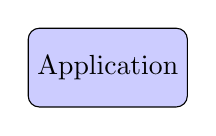
\begin{tikzpicture}
    \node[draw, rounded corners, fill=blue!20, minimum width=2cm, minimum height=1cm] (app) {Application};
  \end{tikzpicture}
  \caption{Demo}
  \label{fig:intro:tikz-demo}
\end{figure}